\documentclass{article}
\usepackage{epigraph}
\usepackage{amsmath}
\usepackage{multirow}
\usepackage{pgf-pie}
\usepackage{pgfplots}
\usepackage{pgfplotstable}
\usepackage{adjustbox}
\title{
    Proportional Representation\\
    \large in the context of it's proposed implementation in the United States}
\author{David G. Boers}

\begin{document}
    \maketitle

    \epigraph{[A legislature] should be in miniature, an exact portrait of the people at large. It should think, feel, reason, and act like them. That it may be the interest of this Assembly to do strict justice at all times, it should be an equal representation, or in other words equal interest among the people should have equal interest in it.}{John Adams}

    \section{Introduction}

    Proportional Representation is a voting system used in over 100 countries to elect people to varius offices. It has many different implementations, families, and method groups. In this essay, I will explain each, and why I chose the rules that I did to propose for use in the United States, in the form of my proposal: "The New Electoral College".

    \section{Basics}

    Many countries, including the United States, use a single-winner voting system called First-Past-the-Post. Under this system, districts are created, and each one elects a single representative. Voters may allocate a single vote to the candidates on the ballot, and the candidate who recives the highest number of votes wins.\\

    Other countries have replaced this system with Proportional Representation. The most common implementation, the Party-List system, involves the abolition of the single-member districts, which are replaced with larger multi-member constituencies. These often reflect a countries first level administrative divisions, like states or provinces. In other cases, countries will designate other constituencies, or combine the whole country into a single-nationwide constituency.\\

    Under Proportional Representation, voters vote for a party, rather than a candidate. The avaliable seats are distributed proportionaly, with approxomatly the same ratio as the votes were cast in.\\

    \section{Party-List Proportional Representation}

    In the Party List system, each party publishes a list of their candidates, with a rank assigned to each candidate. Members are chosen for a party in assending order of the ranks on the list. If a party recives 6 seats, the first 6 names on the list are chosen.\\

    There are ten different methods used to allocate seats under the Party List system. Nine of these are sorted into two families, with an additional method being a mix of the two.\\

    In fact, there are many different methods of Proportional Representation by name, but many are mathematicly identical, produce the same results, or are called different things in different places.\\

    \subsection{Largest Remainder Method (LRM)}

    The Largest Remainder Method (LRM) is also known as Vinton's method, the Hare-Niemeyer method, or Hamilton's Method.\\

    It's calculation process involves a quota. Each party's vote total is divided by this quota, with the respective party winning a seat for every time their total can be evenly divided by the quota. Extra seats are then awarded to parties based off of the remainder of votes.\\

    \subsubsection{Hare Quota}

    The Hare Quota, also known as the Simple Quota, is represented as:

    \begin{align}
        \left \lfloor \frac{\text{total valid poll}}{\text{seats}} \right \rfloor
    \end{align}

    The \textit{total valid poll} is the number of votes cast in an election that count. This excludes ballots where more than one vote was cast, or where no option was marked.\\

    This quota is the most commonly used for Largest Remainder Methods, because of it's simplicity. It is quite easy for voter's to understand how this method allocates seats.

    \subsubsection{Droop Quota}

    The Droop Quota is named after English lawyer and mathematician Henry Richmond Droop. 

    \begin{align}
        \left \lfloor \frac{\text{total valid poll}}{\text{seats} + 1} \right \rfloor + 1
    \end{align}

    The quota is the Hare Quota for an election with one more seat than avaliable, raised by an additional one. It is always smaller than the Hare Quota, resulting in a smaller threshold to win one seat. Despite this, the Droop Quota is known to benefit larger parties over smaller ones. This Quota is critized because of it's apparently arbitrary number. Under some circumstances, it can be more proportional than the Hare Quota. These circumstances are virtually impossible to predict, meaning that there is no difinitive answer to whether the Hare or Droop Quotas are more proportional. The choice should be made based off whether it would be more adivisable to benefit smaller parties, and therefore increase the likleyhood of coalitions, or benefit larger parties.

    \subsubsection{Hagenbach-Bischoff Quota}

    The Hagenbach-Bischoff Quota is represented as follows:

    \begin{align}
        \left \lfloor \frac{\text{total valid poll}}{\text{seats} + 1} \right \rfloor
    \end{align}

    The quota is identical to the Droop Quota, except that an additional one is not added at the end. It is the third largest quota. Usually, the Hagenbach-Bischoff and Droop quotas produce identical results. They both usually favor larger parties over smaller ones. The Hagenbach-Bischoff Quota will, on very rare occasions, allocate more seats than are avaliable. This is mathematically impossible under the Hare or Droop quotas.\\
    
    The Hagenbach-Bischoff quota is sometimes known as the Newland-Britton quota. It is names for it's inventor, Swiss professor Eduard Hagenbach-Bischoff. It is not to be confused with the Hagenbach-Bischoff method.\\

    This is the only quota where it is guarenteed that a party that recives under 50\% of the votes will also recive under 50\% of the seats.

    \subsubsection{Imperiali Quota}

    The Imperiali Quota, not to be confused with the Imperiali method, is the smallest of the quotas.

    \begin{align}
        \left \lfloor \frac{\text{total valid poll}}{\text{seats} + 2} \right \rfloor
    \end{align}

    It is the same as the Hagenbach-Bischoff quota, except two seats are added rather than one. It is uncommon, but possible for the Imperiali quota to elect more representatives than are avaliable. In this case, it is common to increase the quota until the number of seats is corrected.\\

    The Imperiali quota was named after Belgian senator Pierre Imperiali. It benefits larger parties.

    \subsection{Highest Averages Method (HAM)}

    The Highest Averages Method is calculated differently than the Largest Remainder Method. Each of the Highest Averages Methods (of which there are five) have a distinct divisor sequence. Each parties' votes are divided by each divisor sequence, and the top values result in the respective party winning a seat.\\

    \subsubsection{D'Hondt method}

    \subsection{Naming}

    Below is a difinitive list of the methods, and their varius aliases.\\

    \begin{adjustbox}{center}
        \begin{tabular}{ |l|l|l|l|l|l|l| }
            \hline
            Family & Quota/Divisors & Benefits & Names & Namesakes \\
            \hline
            \multirow{2}{*}{Largest Remainder Method} & 
            $ \left \lfloor \frac{\text{v}}{\text{s}} \right \rfloor $ & 
            Smaller Parties & 
            Hare Quota, Simple Quota & 
            Thomas Hare\\
            \cline{2-5}
            & 
            $ \left \lfloor \frac{\text{v}}{\text{s} + 1} \right \rfloor + 1 $ & 
            Larger Parties &
            Droop Quota &
            Henry Richmond Droop\\
            \cline{2-5}
            & 
            $ \left \lfloor \frac{\text{v}}{\text{s} + 1} \right \rfloor $ & 
            Larger Parties &
            Hagenbach-Bischoff Quota, Newland-Britton Quota &
            Eduard Hagenbach-Bischoff\\
            \cline{2-5}
            & 
            $ \left \lfloor \frac{\text{v}}{\text{s} + 2} \right \rfloor $ & 
            Larger Parties &
            Imperiali Quota &
            Pierre Imperiali\\
            \hline
            \multirow{2}{*}{Highest Averages Method} & 
            $ n + 1 $ & 
            Larger Parties & 
            D'Hondt method, Jefferson method & 
            Victor D'Hondt, Thomas Jefferson\\
            \cline{2-5}
            & 
            $ 2n + 1 $ & 
            Smaller Parties &
            Sainte-Laguë method, Webster method &
            André Sainte-Laguë, Daniel Webster\\
            \cline{2-5}
            & 
            $ \frac{1}{2}(n + 2) $ & 
            Larger Parties &
            Imperiali method &
            Pierre Imperiali\\
            \cline{2-5}
            & 
            $ n $ & 
            Smaller Parties &
            Adams method &
            John Quincy Adams\\
            \cline{2-5}
            & 
            $ \sqrt{n(n + 1)} $ & 
            Smaller Parties &
            Huntington-Hill method, Method of Equal Proportions &
            Edward Vermilye Huntington, Joseph Adna Hill\\
            \cline{2-5}
            & 
            $ 2^n $
            & 
            Smaller Parties &
            Macanese method &
            Macau\\
            \hline
        \end{tabular}
    \end{adjustbox}

    \subsection{Calculation Differences}

    To see how each method calculates differently, we will use an example with six parties. The votes are shown below.

    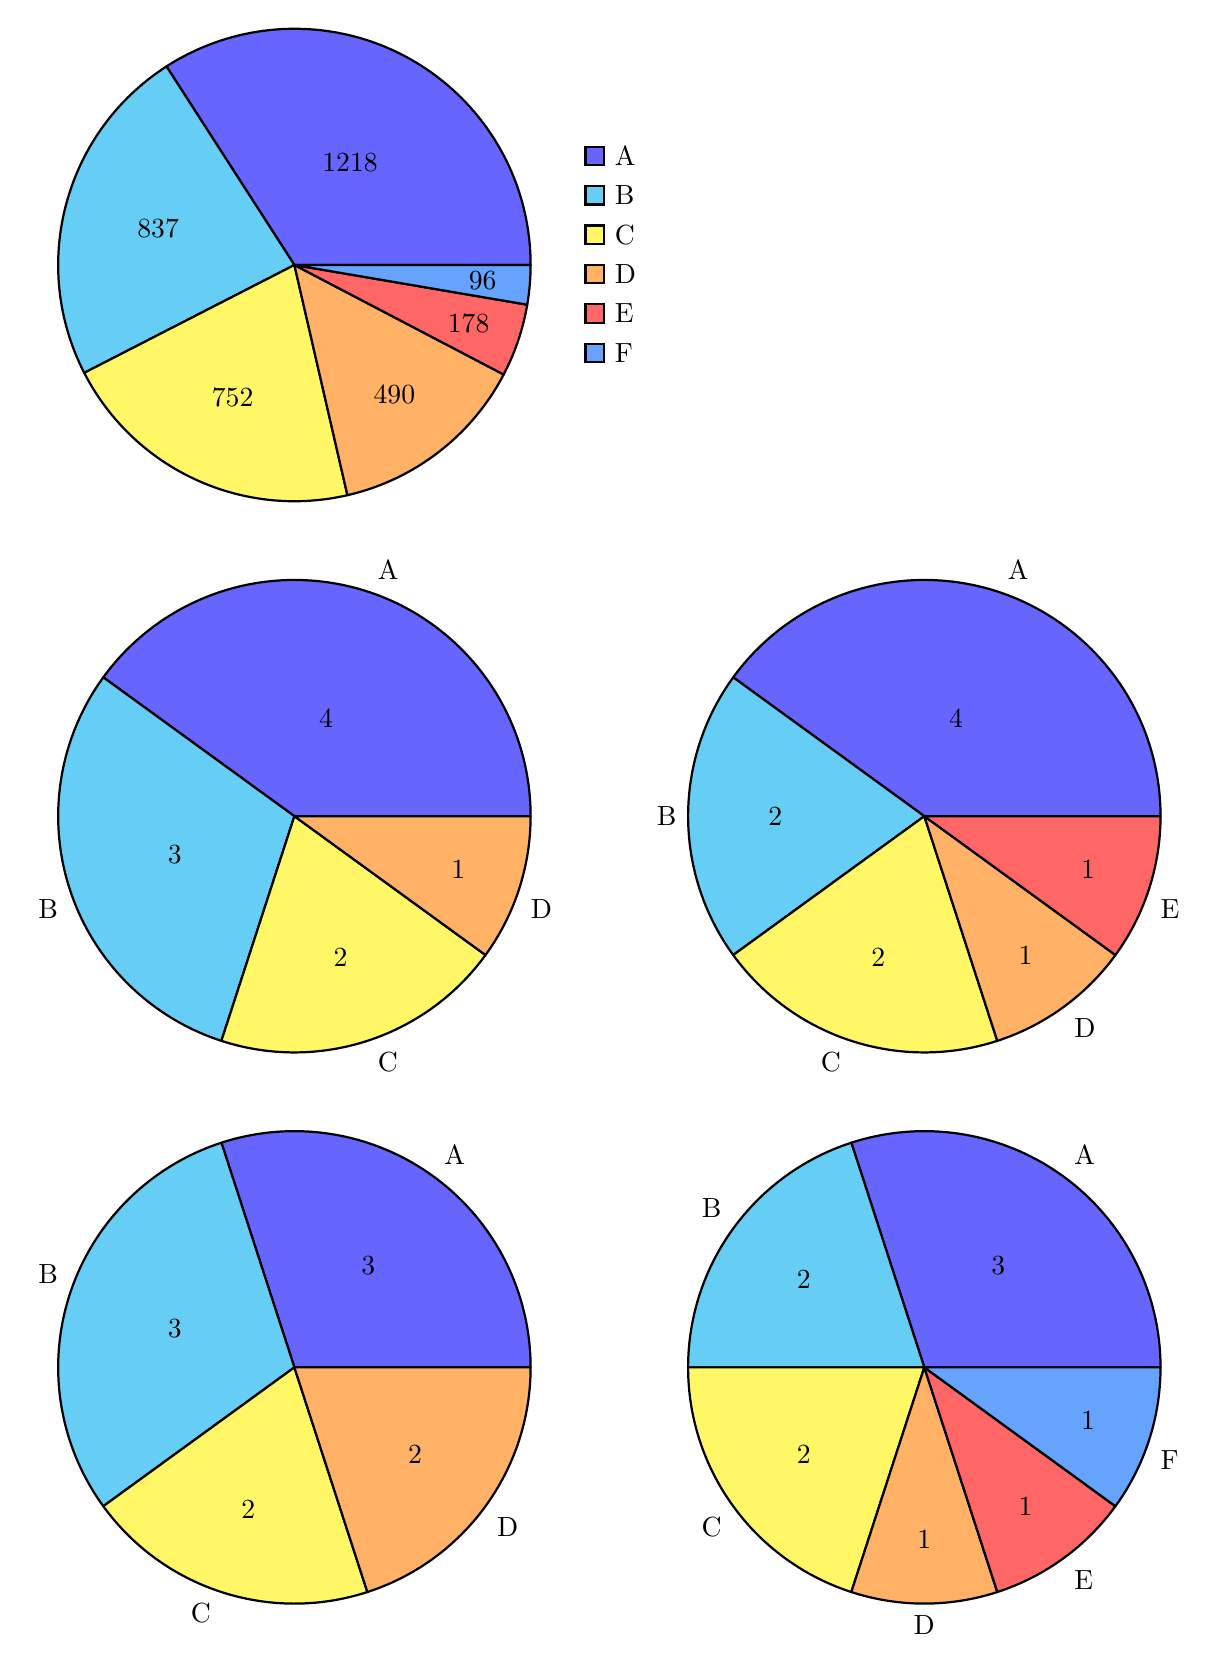
\begin{tikzpicture}
        \pie[pos={0, 0}, sum=auto, text = legend]{
            1218/A,
            837/B,
            752/C,
            490/D,
            178/E,
            96/F
            }

        \pie[pos={0,-7}, sum=auto]{
            4/A,
            3/B,
            2/C,
            1/D
            }
        
        \pie[pos={8, -7}, sum=auto]{
            4/A,
            2/B,
            2/C,
            1/D,
            1/E
            }

        \pie[pos={0,-14}, sum=auto]{
            3/A,
            3/B,
            2/C,
            2/D
            }
            
        \pie[pos={8,-14}, sum=auto]{
            3/A,
            2/B,
            2/C,
            1/D,
            1/E,
            1/F
            }
    \end{tikzpicture}

    Top-left, D'Hondt, Imperiali (Both), Droop, Hagenbach-Bischoff.
    Top-right, Sainte-Laguë, Hare.
    Bottom Left, Macanese.
    Bottom Right, Adams, Huntingon-Hill.\\

    In this particular instance, the allocation determined by the Sainte-Laguë and Hare methods are the most accurate.\\

    Now lets see the same example, but with 50 seats rather than 10.\\

    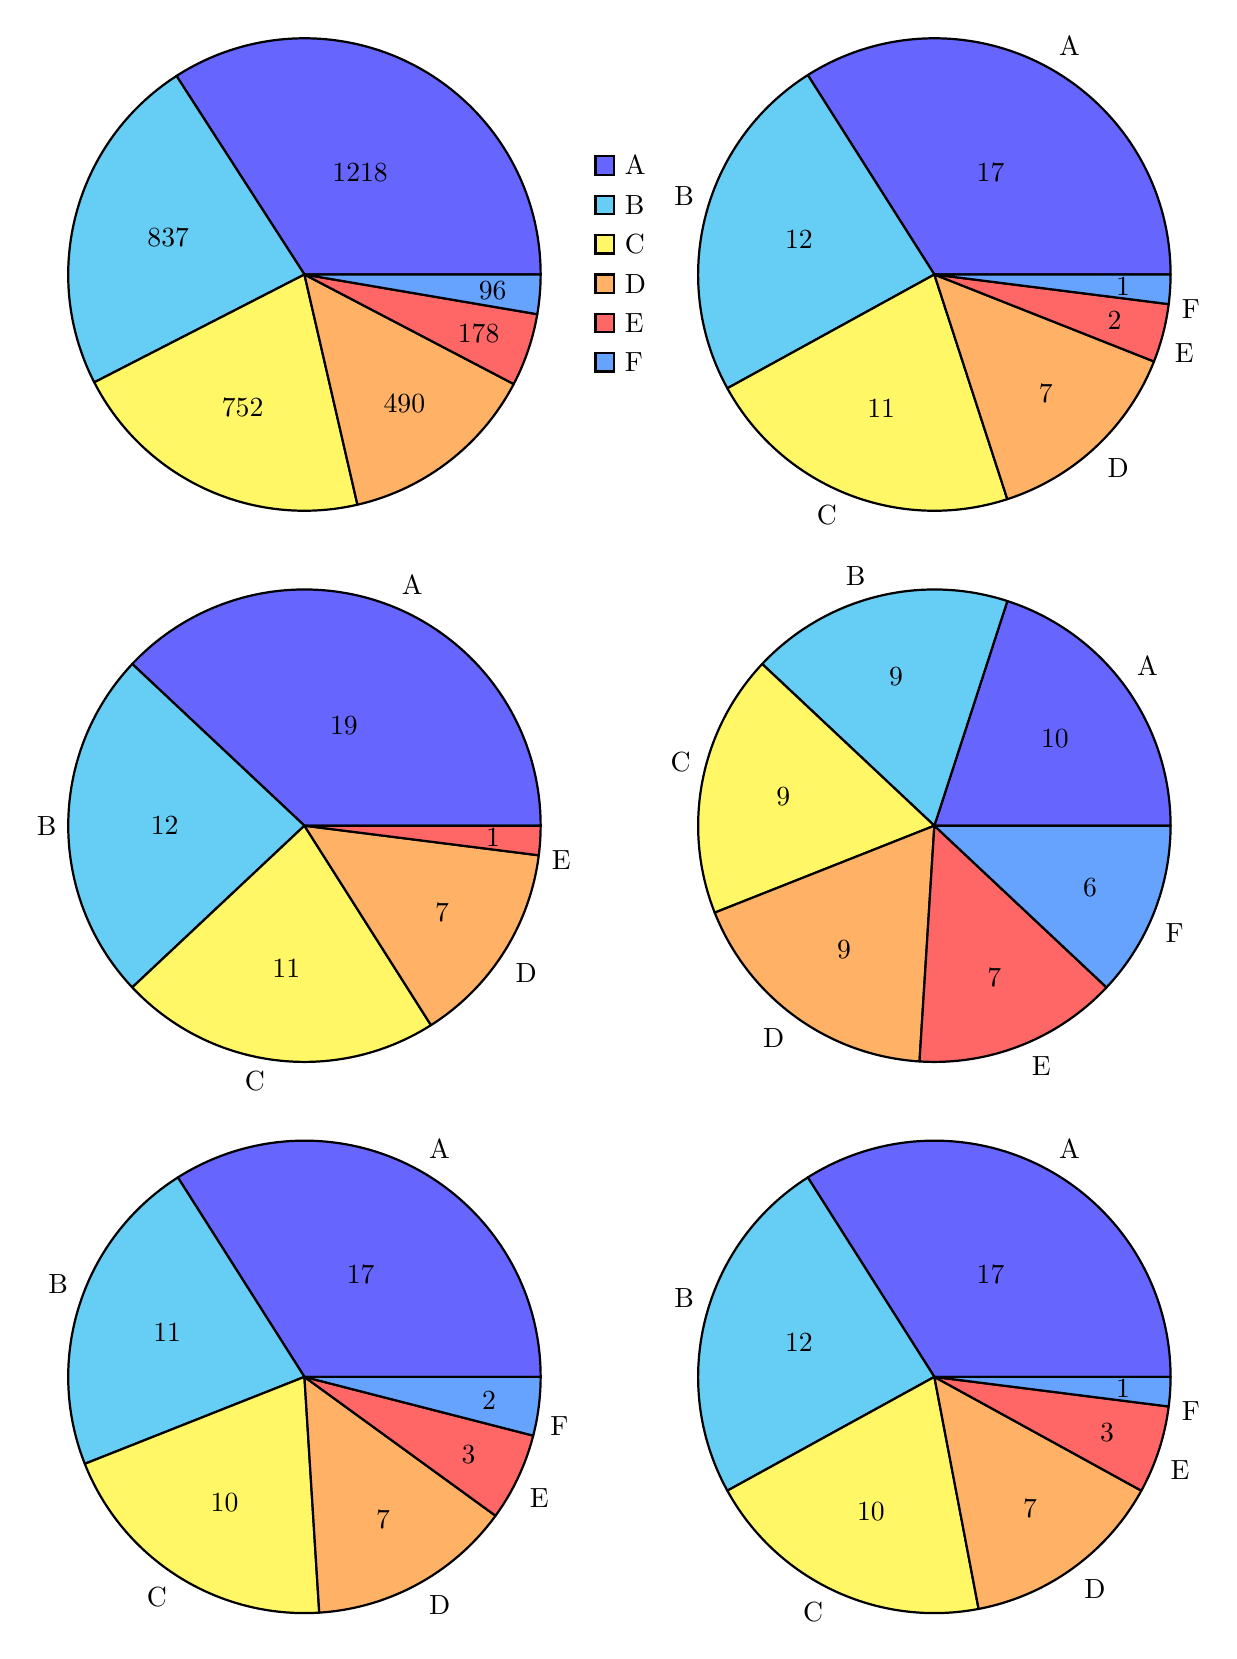
\begin{tikzpicture}
        \pie[pos={0, 0}, sum=auto, text = legend]{
            1218/A,
            837/B,
            752/C,
            490/D,
            178/E,
            96/F
            }

        \pie[pos={8,0}, sum=auto]{
            17/A,
            12/B,
            11/C,
            7/D,
            2/E,
            1/F
            }
        
        \pie[pos={0,-7}, sum=auto]{
            19/A,
            12/B,
            11/C,
            7/D,
            1/E
            }

        \pie[pos={8,-7}, sum=auto]{
            10/A,
            9/B,
            9/C,
            9/D,
            7/E,
            6/F
            }
            
        \pie[pos={0,-14}, sum=auto]{
            17/A,
            11/B,
            10/C,
            7/D,
            3/E,
            2/F
            }
        
        \pie[pos={8,-14}, sum=auto]{
            17/A,
            12/B,
            10/C,
            7/D,
            3/E,
            1/F
            }
    \end{tikzpicture}

    Top-Right, D'Hondt, Sainte-Laguë, Hare, Droop, Hagenbach-Bischoff, Imperiali (LRM).
    Center-Left, Imperiali (HAM).
    Center-Right, Macanese.
    Bottom-Left, Adams.
    Bottom-Right, Huntington-Hill.\\

    Although the number of combinations increases to five, six of the methods agree on one allocation combination. The D'Hondt, Sainte-Laguë, Hare, Droop, Hagenbach-Bischoff, and Imperiali (LRM) methods produce the most proportional result. When the number of seats increase, methods usually differ less in their results. The exception is the Macanese method. When less than 10 seats are filled, the Macanese method performs adiquatly. As the number of seats increase, it produces such skewed results it would strain the definition of "Proportional."\\

    The Macanese method is unique to Macau, the Special Adiminstrative Region of the People's Republic of China. It is likley used here in an attempt to split the anti-Beijing movement into multiple parties, making it difficult to create a unified pro-democracy front.

    \subsection{How Highest Averages Methods advantage parties}

    The faster a sequence of divisors increase, the faster the number of votes decreases. Take a party with 1,000 votes, and an opponent party with 400 votes. Party A would be awarded the first seat under the D'Hondt method and the Sainte-Laguë method. Next, the quotient for Party A would become 500 under the D'Hondt method, and 333.33 under the Sainte-Laguë method. This means D'Hondt would allocate the second seat to Party A, and Sainte-Laguë would allocate it to Party B. The second divisor under D'Hondt is 2, while it is 3 under Sainte-Laguë.\\

    Below is a plot of the divisor sequences.

    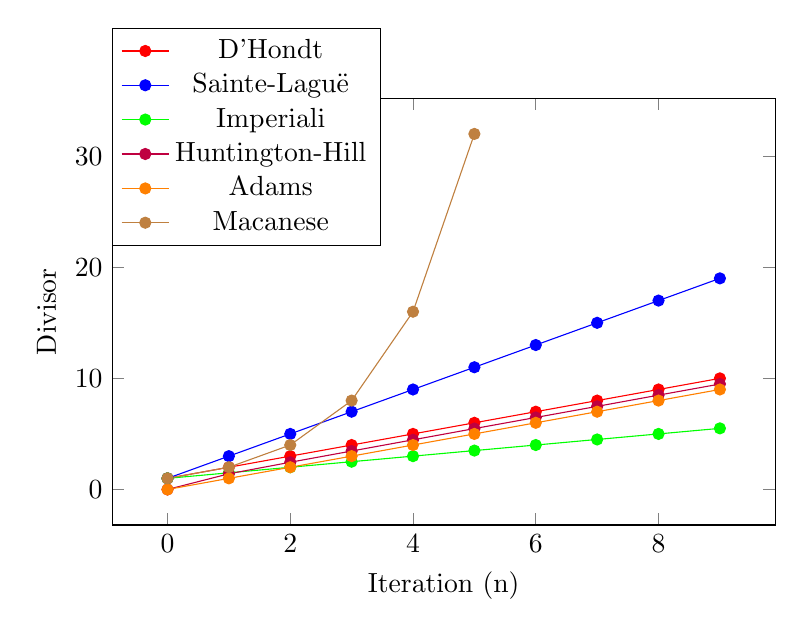
\begin{tikzpicture}

        \begin{axis}[
            xlabel = Iteration (n),
            ylabel = Divisor,
            width=10cm,height=7cm,
            legend style={at={(0.0,.91)},anchor=west}
        ]

        \addplot[color=red,mark=*] coordinates {
            (0, 1)
            (1, 2)
            (2, 3)
            (3, 4)
            (4, 5)
            (5, 6)
            (6, 7)
            (7, 8)
            (8, 9)
            (9, 10)
        };

        \addplot[color=blue,mark=*] coordinates {
            (0, 1)
            (1, 3)
            (2, 5)
            (3, 7)
            (4, 9)
            (5, 11)
            (6, 13)
            (7, 15)
            (8, 17)
            (9, 19)
        };

        \addplot[color=green,mark=*] coordinates {
            (0, 1)
            (1, 1.5)
            (2, 2)
            (3, 2.5)
            (4, 3)
            (5, 3.5)
            (6, 4)
            (7, 4.5)
            (8, 5)
            (9, 5.5)
        };

        \addplot[color=purple,mark=*] coordinates {
            (0, 0)
            (1, 1.41)
            (2, 2.45)
            (3, 3.46)
            (4, 4.47)
            (5, 5.48)
            (6, 6.48)
            (7, 7.48)
            (8, 8.49)
            (9, 9.49)
        };

        \addplot[color=orange,mark=*] coordinates {
            (0, 0)
            (1, 1)
            (2, 2)
            (3, 3)
            (4, 4)
            (5, 5)
            (6, 6)
            (7, 7)
            (8, 8)
            (9, 9)
        };

        \addplot[color=brown,mark=*] coordinates {
            (0, 1)
            (1, 2)
            (2, 4)
            (3, 8)
            (4, 16)
            (5, 32)
            %(6, 64)
            %(7, 128)
            %(8, 256)
            %(9, 512)
        };

        \legend{D'Hondt,Sainte-Laguë,Imperiali,Huntington-Hill,Adams,Macanese}
        \end{axis}
    \end{tikzpicture}

    \subsection{Adams and Huntington-Hill free seat policy}

    The Adams and Huntington-Hill methods have 0 as their first divisor. As it is not possible to divide by zero, the first quotient for each party is given as infinity. Because infinity will always be one of the Highest Averages, each party will get a seat, no matter how small their vote count.\\

    This can sometimes by of advantage. The process of allocating seats to states in the House of Representatives is undertaken using the Huntington-Hill method. Because each state is constitutionaly guarenteed a single seat, most Proportional Representation methods will not surfice.\\

    Sometimes, a threshold is put in place to limit the parties that may gain a seat. Parties that cross a Hare Quota of the votes, for instance, are eligible to gain seats.\\

\end{document}